%code kommentieren, tau, rechtschreibung, 
\documentclass[12pt]{article}
\usepackage{wrapfig}
\usepackage{siunitx}
\usepackage[utf8]{inputenc}
\usepackage[english]{babel}
\usepackage{graphicx}
\usepackage{hyperref}
\usepackage{xcolor}
\hypersetup{
    colorlinks=true,
    linkcolor=black,
    filecolor=black,
    urlcolor=cyan,
}
\urlstyle{same}
\author{{\Huge Carl Jonas Mikaelsson Berggren}}
\font\myfont=cmr12 at 30pt
\title{{\myfont Spezielle Relativität}}

\begin{document}
\maketitle
\tableofcontents
\newpage
\begin{abstract}
In diesem Dokument erkläre ich, wie ich ein Programm entwickelt habe, was Albert Einsteins spezielle Relativität visualisiert.
Das Programm Arbeitet anhand von Minkowski-Raumzeitdiagrammen, und nutzt Objektorientierte Programmierung.

Außerdem Erkläre ich die darunter liegende Physik und leite Lorentztransformation her.
Dabei werde ich auf Relativität vor Einstein, auf Minkowski-Raumzeit-Diagramme, auf Transformationen zwischen Bezugssystemen, Auf die Implikation Spezieller Relativität, und dessen Einschränkungen.
Dabei beziehe ich mich nur auf spezielle Relativität und nehme inertiale Bezugssysteme in einer flachen Raumzeit an.
\end{abstract}
\section{Relativität nach Newtonscher Physik}
Bevor wir über Einsteins spezielle Relativität reden können, müssen wir das Konzept von Raum, Zeit und Bewegung klarstellen
\subsection{Bezugssysteme}
%position Rotation Zeit, Geschwindgikeit
Zunächst muss klar gestellt werden wie Position, Zeit und Geschwindigkeit gemessen werden.
Dazu muss ein Koordinatensystem räumlich und zeitlich definiert werden.
Dass Koordinatensystem hat einen Ursprung  mit $x = y = z = t = 0$.
Hierbei liegt der Ursprung des Koordinatensystems in der Regel auf ein Objekt zu Beginn des Beobachtungszeitraums bezogen.
Durch die Tatsache, dass in allen Inertialen Bezugssystemen die gleichen physikalischen Gesetze gelten, sind alle Bezugssysteme gleich gültig.
Es ist keine universal-gültige Aussage über die Position oder Geschwindigkeit eines Körpers, oder Zeitpunkt eines Ereignisses möglich.
Demnach ist es Bedeutungslos zu sagen, man hätte zum Zeitpunkt $t$ die Position $x, y, z$ und bewege sich mit einer Geschwindigkeit $\vec{v}$.
Es muss immer ein Bezugspunkt gewählt werden z.b. Erdmittelpunkt, Upload des ersten http Dokuments.
Bezugssysteme können sich also relativ zu eine ander bewegen und dennoch gleichermaßen gültig, das selbe Ereignis beschreiben.
\subsection{Galilei-Transformation}
Ich werde mich im folgenden auf eine Raumdimension beschränke.
Weitere Raumdimension können durch ersetzen der gerichteten Größen durch Vektoren hinzugefügt werden.
$x$ wird demnach zu $\vec{0p}$, $v$ zu $\vec{v}$.
Dabei ist zu beachten, dass die gerichteten relativistischen Effekte nur endlang der Bewegungsrichtung auftreten.
Wie dies funktioniert wird in Abschnitt \ref{4v} näher erläutert.

Es wird zunächst ein bezugssystem gewählt mit den Größen $x, t$ und $v$.
Anschließend wir ein gestrichenes Bezugssystem gewählt mit den Größen $x', t'$ und $v'$, wobei $t = t'$ gilt.
Aus unserer alltäglichen Erfahrung geht hervor, dass für die Position eines, zu dem ungestrichenen Sytstem statischen Objekt gilt: 
\begin{equation}
x' = x-vt
\end{equation}
Genau so gilt für Geschwindigkeiten:
\begin{equation}
\label{vnewton}
u' =u - v
\end{equation}
Hierbei ist v die Geschwindigkeit des gestrichenen Bezugssystems und $u$ Die Geschwindigkeit des betrachteten Objekts.

\begin{wrapfigure}{R}{0.4\textwidth}
\centering
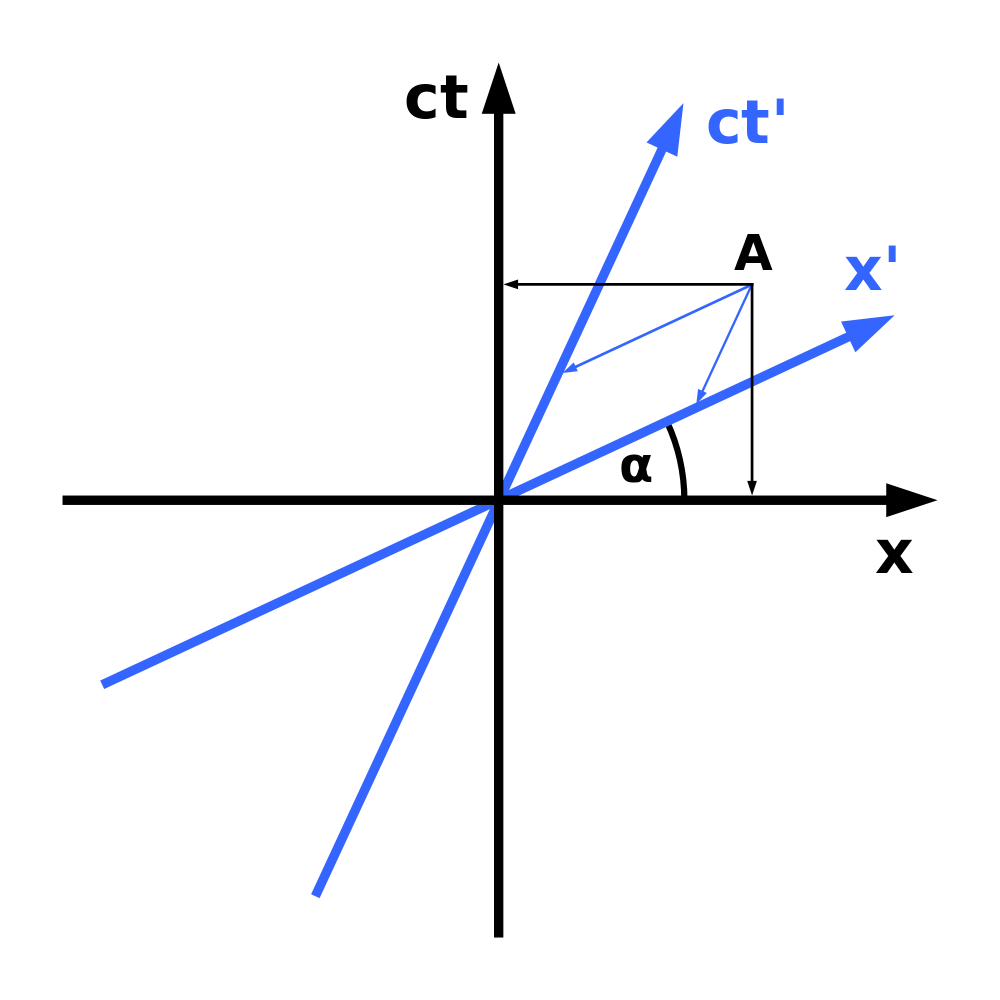
\includegraphics[width=0.3\textwidth]{Minkowski_diagram.png}
\end{wrapfigure}
\subsection{Minkowsky-Raumzeitdiagramme}
Das Minkowski-Raumzeitdiagramm betrachtet, in seiner üblichen Form, Objekte in einer Raumdimension und Zeit.
Hierzu wird die Zeit auf die vertikale Achse gelegt und die Position auf die horizontale.
Für die Betrachtung von spezieller Relativität werden die Einheiten einfachheitshalber so gewählt, dass für die Lichtgeschwindigkeit $c = 1$ und $x = ct$ gelten.
Objekte werden als Gerade Dargestellt und Ereignisse als Punkte.

\section{spezielle Relativität}
%spacelike, timelike
%lightcone
Die spezielle Relativität fügt ein entscheidendes Postulat hinzu:
\begin{itemize}
\item Die Lichtgeschwindigkeit ist ein universelle Konstante
\end{itemize}
Dies wirft direkt eine Frage auf:
Wenn jemand mich mit einer Taschenlampe anleuchtet während ich mich auf ihn zu bewege, wie kann es dann sein, dass wir beiden den exakt gleichen wert für die Geschwindigkeit diese lichts messen?
Wenn eine Einzelne Geschwindigkeit immer identisch ist ist es unmöglich, dass Raum und Zeit erhaltene Größen sind.
\subsection{Herleitung}
\label{herl}
Es werden zwei Bezugssysteme betrachtet, die sich relativ zu einander mit der Geschwindigkeit $v \neq 0$ bewegen.
In dem ungestrichenen Bezugssystem fliegt ein Photon zwischen zwei Spiegeln hin und her, die eine Strecke $l$ von einander entfernt sind.
Um von einem Spiegel zum anderen zu gelangen muss das licht vom gestrichen System aus gesehen eine Größere Strecke $d$ zurücklegen, nämlich:
\begin{equation}
d^2 = l^2 + (vt')^2
\end{equation}
Da $d \neq l$ gilt, jedoch beide Strecken mit der gleichen Geschwindigkeit zurückgelegt werden, muss $\Delta t' \neq \Delta t$ gelten.
Drückt man $d$ und $l$ in $c$ aus so gilt:
\begin{equation}
c^2 \Delta t'^2 = c^2 \Delta t^2 + v^2 \Delta t'^2
\end{equation}
Dies kann dann durch substrahieren von $v^2 \Delta t'^2$ um ausklammern von $t'^2$ nach $t'$ aufgelöst werden.
Dann gilt:
\begin{equation}
\Delta t' = \frac{\Delta t}{\sqrt{1-\frac{v^2}{c^2}}}
\end{equation}
Teilt man nochmal durch $\Delta t$, ergibt sich der Relativitätsfaktor $\gamma$:
\begin{equation}
\label{gamma}
\gamma = \frac{1}{\sqrt{1-\frac{v^2}{c^2}}}
\end{equation}
\subsection{Transformation zwischen Bezugssystemen}
\label{trans}
Dies löst aber nicht direkt die Frage der Geschwindigkeitsaddition.
Das Postulat ist nämlich nicht mit der Formel \ref{vnewton} vereinbar.
Geschwindigkeitsaddition muss daher neu definiert werden und zwar als:
\begin{equation}
\label{v}
v' = \frac{u + v}{1 + \frac{uv}{c^2}}
\end{equation}
Es gelten außerdem:
\begin{equation}
t' = \gamma(t \frac{vx}{c^2})
\end{equation}
\begin{equation}
x' = \gamma(x + vt)
\end{equation}
$t$ und $x$ beschreiben die Position und den Zeitpunkt eines Ereignisses.
Hingegen beschreibt $\Delta t$ aus Abschnitt \ref{herl} einen Zeitabstand.
\subsection{Raumzeititnerval als erhaltene Größe}%in 4v einbauen
%Formulierung checken
Nach der speziellen Relativität sind Raum, Zeit und sogar die Reihenfolge von ereignissen relativ.
Es wirkt so als nur die Lichgeschwindigkeit konstant.
Es gibt aber eine weiter Größe die unter Lorenztransformation invariant bleibt:
Die sogenannte Eigenzeit%Raumzeitinterval
\begin{equation}
\tau^2 = (\Delta ct)^2 - {\Delta x}^2 - {\Delta y}^2 - {\Delta z}^2
\end{equation}
Wobei $\Delta t$der Zeitlcihen und $\Delta x, y, z$ den räumlihen Abstand zwisch zei ereignisse darstellen.
$\tau$ kann im Minkowski-Diagramm als Vektor dargestellt werde der die Ereignisse verbindet.

Diese Größe kann durch die Kombination aus negativen Raumkomponente uns positiver Zeitkomponenten im gesamten Reellen bereicih definiert.
Was für ein Wert diese Größe hat hat aufwirhung darauf worüber sich beobachter uneinig sein können.

Ist $\tau$ negativ können sich Beobachter über die Reinfolge der Ergnisse uneinug sein.
Außerdem können sich die beiden Ereignisse nicht beeinflussen.
Dies ist im Diagramm daran zu erkennen, dass der Winkel zwischen $\tau$ und der $ct$-Achse kleiner als \ang{45} ist.
Somit sind auch Gleichzeitigkeitslinien zulässig die Steiler sind als $\tau$.
Weltlinien die flacher sind als $\tau$ sind jedoch unzulässig

Gilt $\tau = 0$ so kann das eine Ereigniss das ander durch ein Lichtteilchen beinflussen, jedoch nicht durch ein massebehaftetes Signal.

Ist $\tau$ positiv ist die Reinfolge der Ereignisse unversell.
In dem Fall entspricht $\tau$ der Zeit die eine Uhr zwischen den Ereignissen messen würde, die sich von dem ersten zu den zweiten Ereignis bewegt
.%proper wenn tau > 0
\subsection{Vierervektoren und Vierergeschwindigkeiten}
%Matrix
\label{4v}
Vorweg etwas zur Notation: 4-dimensionale Vektoren haben den tiefgestellte Index $\mu$ während 3-dimensional euklidische Vektore $i$ stattdessen haben.
Vierervektoren, oder auch 4-Vektoren, stellen eine Móglichkeit dar Speziele Relativität auf alle drei Raumdimensionen anzuwenden.
Hierzu wird einem Vektor eine Zeit-Komponente Hinzugefügt.
\begin{equation}
X_\mu = (c\Delta t, \Delta x, \Delta y, \Delta z)
\end{equation}
Der Raum der 4-Vekoren verhält sich ähnlich wie der Raum der gewöhnlichen Vektoren.

Die Geometrie Entspricht hier jedoch nicht mehr der Euklidischen Geometrie sondern der Minkowski-Metrik.
Der Maßgebliche unterschied besteht darin, dass Abstände nicht als $\sqrt{\Delta a_1^2 + \Delta a_2^2 + ... + \Delta a_n^2}$ definiert sind sondern als $\sqrt{\Delta a_1^2 - \Delta a_2^2} - ... - \Delta a_n^2$.%hier tau einbauen
Somit sind Negatiev Abstände möglich.
Außerdem können so ungleiche Punkte dennoch einen Abstand von 0 aufweisen.
Skalare sind in dem Zusammenhand auch anders definiert.
Skalare sind nun alle physikalischen Größen die in allen Bezugsystemen identisch sind.
Dies sind zum Beispiel $\tau$ zwischen zwei Ereignissen.%weitere

Mit 4-Vektoren sind die selben Operationen möglich wie mit normalen 3-dimensionalen Vektoren.
Allerdings sind sie auf Grund der Minkowski-Metrik anders definiert.
%transformationmatrix
Für Skalarmultplikation zwischen Vektoren git:
\begin{equation}
	a_\mu \cdot b_\mu = a_0 b_0 - a_1 b_1 - a_2 b_2 - a_3 b_3
\end{equation}
Demnach gilt außerdem:
\begin{equation}
X_\mu ^2 = (c\Delta t)^2 - \Delta x^2 - \Delta y^2 - \Delta z^2 = \tau^2
\end{equation}

Multipliziert man 4-Vektoren mit einander ist das Ergenis immer ein Skalar.
Multpliziert man 4-Vekoren imt Skalaren ist das Ergebnis ein 4-Vektor.

Ähnlich wie in der Euklidischen Geomtrie $\vec{v} = \frac{\vec{s}}{t}$ gilt, Gilt f dei 4-Geschwindigkeit:
\begin{equation}
	U_\mu = \frac{X_\mu}{\tau} = \gamma(|u_i|) (c,u_i)
\end{equation}
Dies stellt den Bewegungsvektor jedes Objekts durch die Raumzeit dar.
Dabei gilt:
\begin{equation}
u_i = \vec{v}
\end{equation}
Nun soll der Betrag der 4-Geschwindigkeit ermittelt werden.
\begin{equation}
U_\mu ^2 = (\gamma(u))^2(c^2-|u|^2) = \frac{1}{1-(\frac{u^2}{c^2})} (c^2 - u^2)
\end{equation}
erweitert man $\gamma$ um $c^2$ gilt:
\begin{equation}
	U_\mu = \frac{c^2}{c^2 - u^2} c^2 - u^2 = c^2 \frac{c^2 - u^2}{c^2 - u^2} = c^2
\end{equation}
\begin{equation}
	|U_\mu| = \sqrt{U_\mu^2} = c
\end{equation}
Dies bedeutet, dass sich alles mit Lichtgeschwindigkeit durch die Raumzeit bewegt.
Steht man still hat diese Bewegung nur eine Zeitkomponente.
Bewegt man sich jedoch mit Lichtgeschwingkeit durch den Raum ist die Zeitokompente der Bewgung gleich 0.
\begin{wrapfigure}{R}{0.5\textwidth}
\centering
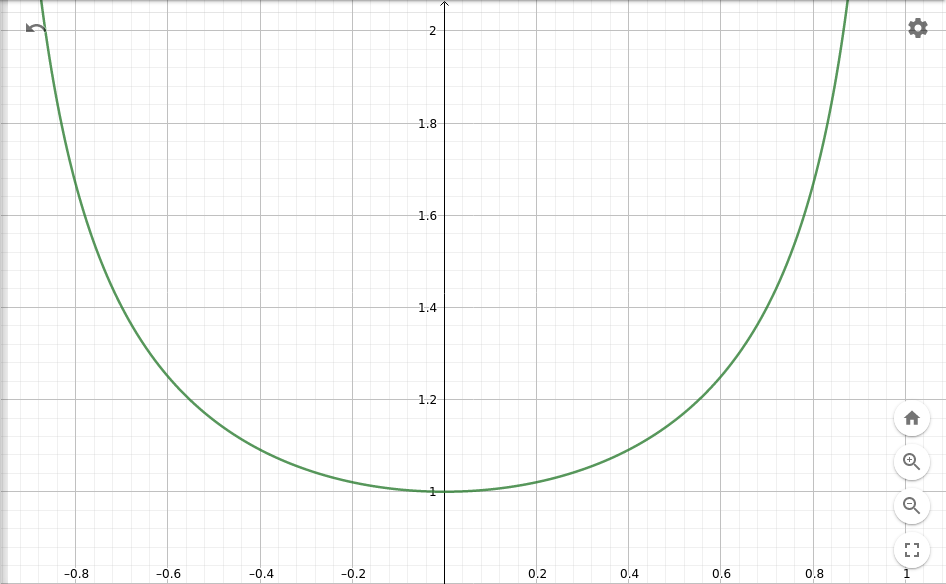
\includegraphics[width=0.4\textwidth]{gamma.png}
\end{wrapfigure}
\subsection{Implikationen}
Dass all diese Effekte nichts mit unserer alltäglichen Erfahrung zu tun haben liegt an Dem Steigungsverhalten von $\gamma$ und der enormen Größen von $c$.
\begin{equation}
c = 299792458 \frac{m}{s}
\end{equation}
Die Parker Solarsonde, eins der schnellsten menchengemachten Objekte, hat eine Geschwindigkeit von etwa $51291 \frac{m}{s} = 1.71 \cdot 10^{-4} c$.
Der Lorentzfaktor für diese Sonder bertägt $\gamma = 1 + 1.5\cdot10^{-8}$.

Deswegen fordert Sspezielle Relativität unster Vorstellungsvermogen immer wiedeer heraus.
Dies wird in einerr Vielzahl von Paradoxen deutlich die sich daraus ergeben.
Alle dieser Pardoxen sind Mathematisch Vergleichsweise einfach zu lösen.

Ein Paradoxon ist zum Beispiel das Tunnel-Paradoxon:
Ein sehr schneller Zug fährt durch ein Tunnel der kürzer ist als der Zug.
An Eingang und Ende des Tunnels befinden sich Tore die sehr schnell geöffnet und wieder geschlossen werden können.
Aus der Perspektive einer Person die neben des Gleisen steht wird der Zug durch den Lorentzfaktor verkürzt.
Dadurch können sich die Tore kurz gleichzeitigscließen ohne, dass es Zum Unfall kommt.
Aus dem Bezugssystem eines Fahrgasts wird jedoch der Tunnel gestaucht.
Daher hätte ein gleichzeitiges schließen der Tore zweifellos katstrophale folgen.
Wie sind diese beiden Beschreibungen vereinbar?
Wir wissen nun aus Abschnitt \ref{trans}, dass Zeit, und gleichzeitigkeit relativ sind.
in dem Beispiel würde der Passnt sehen, dass sich die Tore gleichzeitig schließen.
Für Fahrgast würde sich edoch erst das eine und dann das andere Tor schließen.

Außerdem ergibt sich unter anderem aus der Gleichung \ref{v} eine Geschwidigkeit größer als $c$ unmöglich ist.
Da dies für alle Objekte gilt, somit auch für Information,  ist dies auch die Geschwindigkeit von Kausalität.
\subsection{Einchränkungen dieses Modells}
Spezielle Relativität beschreibt nur inertiale Bezugssysteme in einer Flache Raumzeit.

Inertiale Bezugsysteme sind unbeschleunigt.
Ein Ball der mit einer Geschwindigkeit gleich null losgelassen wird behält seine Position bei.

Dies löst zum Beispiel das bekannt Zwilligspardoxon:
Ein Zwilling Fährt auf eine Raummision bei der er mit beispielsweise halber Lichtgeschwindigkeit durch das All fliegt, während sein Bruder auf der Erde vebleibt.
Als er zur Erde zurückkehrt stellt sich die Frage wer nun älter ist
Nach der Speziellen Relativitität können sich beide Zwillinge für den Zeitraum der mission als statisch betrachten und den anderen als bewegt.
Demnach kommen beide zudem Schluss, dass sie selbs älter sein sollten.

Dabei wird jedoch vernachlässigt, dass der Astronaut beispielsweis zu Alphacentauri fliegt dort umkehrt und wiederkommt.
Dabei erfäht er eine Beschleungiung, die die Spezielle Relativität nicht vorsieht.

Nehme man an der Astronaut führe bei Alphacentauri ein Swingby-Manöver durch und ändere so seine Richtung, so würdeer sich nicht in einer Flachen Raumzeitbewegen.

Diese überlegung führt usn in die Algemeine Relativität, die sich maßgeblich von Newtons Gravitation unterscheidet.
Gravitation wird nicht mehr als Kraftfeld beschrieben sondern als Raumzeitkrümmung, die die inertiale Laufbahn von objekten verändert.

\section{Programm}
Das Programm basiert auf Objekt orientierter Programmierung und mutzt das pygame Modul fur die Grafik.
Ich habe ins gesamt vier Klassen entwickelt:
Eine für die Darstellung der Bezugsstysteme im Diagramm, eine für die Darstellung von buttons und zwei für die Darstellung der Eingabefelder.
Außerdem habe ich jeweils eine Funktion zum wechseln von Bezugssystem,und zum Handhaben von unzulässigen Nutzereingaben.
\subsection{Nutzung}
Diese Programm in python2.7 ausgeführtwerden.
In dem rechten Feld können Geschwindigkeit und Startposisiton von Objekten eigeben werden.
Beim klicken der send-Taste wird die Weltlinie, und die dazu gehörige Gleichzeitigkeitslinie des Objektes in das Koordinatensystem eingezeichnet.
Es können nach belieben Objekte hinzugefügt oder entfernt werden.
Alle sichtbaren Weltlinien kónnen angeklick werden um die Lorentz-Transformation in das jewilige Bezugsystem beobacheten zu können.
\\

Zu Beginn läuft einmalig eine Initialisierungsroutine durch.
Es pygame initialisiert und dann weredn alle globalen Variablen definiert.
diese sind unter anderem Farben, Fenster, Oberfächen, Bilder, Listen, Mathemaatische Funktionen und textinhalte.

Danach werden die Instanzen der Klassen definiert die zu beginn gebraucht werden.
Anschließend staret die Hauptschleife.

Sie beginnt damit durch alle pygameevents zu iterieren.
Wird ein 'Schließen' Signal erfasst wird \colorbox{gray}{running} gleich False gesetzt, und das Programm somit beendet.

Innerhalbdieser Schleife werden die pygaeevents an alle \colorbox{gray}{handle} Mathoden von allen Instanzen übergeben.

Anschließend werden Die Koordinatenachsen gezeichet und die \colorbox{gray}{draw} Methoden von allen Instanzen aufgerufen.

Zuletzt werden die Oberflächen auf das Fenster gezeichnet, das Bild erneuert, die Oberfächen zurückgesetzt.
\subsection{Button}
Die Klasse \colorbox{gray}{Button} dient zur Darstellung und Handhabe aller buttons.
Diese Klasse nimmt einen Typ und optional, einen parent als Argument.
\subsubsection{Methoden}
In dem Konstruktor wird die Box in abhängikeit von Typ definiert.
Anschließend werden weitere Instanzvariablen, für Farbe, Aktivität, Text, Typ, Mutterobjekt definiert.
\\

Die Methode \colorbox{gray}{handle} wird in der Hauptschleife aufgerufen und nimmt pygame ereignisse als Argumente.
In abhängikeit vom Typ wird der Ortsvektor der Maus angepasst.
Wenn sich die Maus über ein dem button befindet wird der Activitäszustand auf True gesetzt, andern Falls auf False.
Jenach Aktivitätszustand wird in der Methode \colorbox{gray}{draw} die Farbe ändert, was ein Hoverfunktion darstellt.
Befindet sich die Maus über \colorbox{gray}{self}, wird dann bei einem Klick, zwische den Typen unterschieden.
Ist \colorbox{gray}{self.type} gleich add, wird der Liste der \colorbox{gray}{objs} eine Instanz von \colorbox{gray}{Obj} hinzugefügt.
Außerdem wird die Position von \colorbox{gray}{self.rect} angepasst.

Ist \colorbox{gray}{self.type} gleich send wird der index von \colorbox{gray}{self} ermittelt, und der Methode \colorbox{gray}{enter} übergeben, die in Abschnitt \ref{inputm} näher erläutert wird.

Ist \colorbox{gray}{self.type} gleich ok wird die globale Variable \colorbox{gray}{err} Nne gesetzt.

Ist \colorbox{gray}{self.type} gleich x wird der index von \colorbox{gray}{self} ermittelt.
Anschleißend wird dieser Index genutzt, um die jeweiligen einträge in dem Listen \colorbox{gray}{objs}, \colorbox{gray}{delbuttons}, \colorbox{gray}{inputs} und \colorbox{gray}{sendbuttons}.
anschließend werden die Position von den verbleibenden Elementen angepasst um das gelöschte Element aufzufüllen.
\\

Die Methode \colorbox{gray}{draw} wird in der Hauptschleife aufgerufen und zeichnet je nach Typ \colorbox{gray}{self.rect} und \colorbox{gray}{self.txt} auf die unterschiedlichen Flächen.
\subsection{Input}
Die Klaase \colorbox{gray}{Input} erstellt Eingabefelder indem sie drei Intsnazen der Klasse Box erstellt.
Der Sinn dieser Klasse ist, die Liste der Eingabefelder besser zu organisieren damit indexe leichter gehandhbt werden kónnen.
\subsubsection{Methoden}
Diese Klasse hat bis auf den Konstruktor nur die Methode \colorbox{gray}{enter}.
Sie beim Klicken des 'send' Buttons aufgerufen.
Sie prüft die Eignaben in dem jeweiligen Feldern auf zulässigkeit.
Es wird überprüft ob Parameter die Zahlen sein sollen Zahlen sind, und das keine Geschwindigkeit über der Lichtgeschwindigkeit eingegeben wird.
Wir ein unzulässige Eingabe erkannt wird die Funktion \colorbox{gray}{err} aufgerufen, die eine Fallspezifische Fehlermeldung anzeigt.
Sind Felder leer, weredn Standardwert ergenzt.
Anschießend wird mit ermittelten den Parametern eine neue Instanz von \colorbox{gray}{Obj} erstellt.
\label{inputm}
\subsection{Box}
Die Klasse \colorbox{gray}{Box} ist die eingentlcihe Maschienrie hinter den Eingabefeldern.
Jenachde was für Parameter übergeben werden, wir \colorbox{gray}{self} zum Namens-, Positions- oder Geschwindiggkeitsfeld.
Demnac werden Position, und Standrdinhalt angepasst.
\subsubsection{Methoden}
Die Methode \colorbox{gray}{handle} wird in der Hauptscheife aufgerufen, und nimmt pygameevents als Parameter.
wird das Feld angeklick, wird Der Standardinhalt entfernt und \colorbox{gray}{self.active} gleich True gesetzt.
Wird woanders hingeklickt, werde sie Veränderungen wieder rückgängig gemacht.
Demanch wird auch die Farbe des Feldes angepasst.
Ist anschließend \colorbox{gray}{self.active} True werden die Tastatureingaben gespeichert.
\\
\colorbox{gray}{draw} Zeigt dann den passenden Text und das Felde in der richtigen Farbe.
\subsection{Obj}
\colorbox{gray}{Obj} ist das Herzstück des Programms.
Es handhabt alle Einträge in das Diagramm.
Es Arguente, die den Namen, den Index, die Position, die Geschwindigkeit, den Farbindex und t = 0 definieren.
Es eren zunächst alle Argumente als Instanzvariablen gespeichert.
Anschließend werden der Winkel der Weltlinien und ie Weltlinie definiert.
anschießend wir \colorbox{gray}{pos} definiert was das errechnen von Punkten Entlang der Weltlinie massiv ereichtert.
Falls der Betrag von\colorbox{gray}{self.v} kleiner als 1 ist werden zusÄtzlich graphisch Features definiert.
Diese sind die Gleichzeitigkeitslinie für t=0, kleine Einheitmarker für x und t und das Gesamte Koordinatensystem für das Jeweilige Bezugsystem.

Für die Gleichzeitigkeitslinie wird eine neue Linie erstel die um 90-\colorbox{gray}{self.angle} rotiert ist.
Für die Einheitsmarker wird der Schnittpunkt zwischen den Beiden Gerade ermittelt.
Von dort ausgehend werden iterativ neue Positionen für entlang der Geraden ermittelt die um eine Konstante $/cdot \gamma$ von einander entfernt sind.

Ähnlich wird auch das Koordinatensystem definiert.
Hier wird jedoch der Referenzpunkt der Geraden als Startpunkt gewählt.

Zuletz wird die Position des Namens definiert.
Der Name Steht immer rechts neben der Weltlinie soweit oben wie es möglich ist ohne das zwei namen kolidieren.
\subsubsection{Methoden}
\colorbox{gray}{draw} prüft ob \colorbox{gray}{self.v} gleich 1 ist.
Wenn das der Fall ist wird nur die Weltlinie gezeichnet.
Andernfall werden mindestens die Einheitsmarker, und die Gleichzeitigkeitslinie hinzugefügt.
Ist \colorbox{gray}{self.active} wird zusätzlich nich das Gesamte Koordinantensystem gezeichnet.
\\

\colorbox{gray}{handle} handhabt das Nutzerverhalten in Bezug auf das Diagramm.
befindet sich die Maus über der Weltlinie, wird \colorbox{gray}{self.active} zu True.
Wir die Weltlinie angeklickt, wird die Funktion \colorbox{gray}{change} aufgerufen, und somit das wechseln des Bezugsystem initiiert.
Wie das Funktioniert ist in Abschnit \ref{func} näher erklärt.
\subsection{Funktionen}
\label{func}
Die Funktion error wird von der Funktion enter bei jedem Fehlerfall aufgerufen.
Es wird ein Fallspezifischer Fehlerwert übergeben.
Die Funktion error erstellt ein Fenster auf dem eine fehlerspezifische Nachricht angezeigt wird.
Außerdem wir ein 'ok' button erstellt mit dem das fenster wieder geschlossen werden kann.
\\

Die funktion \colorbox{gray}{change} wird aufgerufen wenn der Nutzer eine Weltlinie anklickt und danach in jeder Iteration er Programms, bis die Lorenztransformation ferig ist.
Sie nimmt den Index des gewünschten Bezugsystems als Argument.
Die Änderung der Bezugsystems wird der anschauligkeitshalber für jede Größe nacheinander gemacht.
zuerst wird endlang der x-Achse verschoben, dann wird die Geschwindigkeit angepasst und zuletzt t justiert.
Dies alles wird aber nicht in Schleifen in der Funktion gemacht, da so die zwischenschritte zur fertigen Transformation nicht gezeichet werden Würde.
\section{Quellen}
Loedel-Minkowski-Diagramm; zweidimensionale Raumzeit(Zugriff: 06.09.2019):

%\url{https://www.youtube.com/watch?v=mJcRHBviHBI}
\url{https://stackoverflow.com/questions/46390231/how-to-create-a-text-input-box-with-pygame}
\url{https://www.youtube.com/playlist?list=PLD9DDFBDC338226CA}
\url{http://edu-observatory.org/olli/Relativity/Minkowski_diagram.png}
\url{https://www.youtube.com/playlist?list=PLDB7DB12B34395EC5}
\end{document}
